\section{Auswertung}
\label{sec:Auswertung}
In diesem Kapitel werden alle gemessenen Daten ausgewertet.
\subsection{Überprüfung der Bragg-Bedingung}
\label{sec:Braggbedingung}
Im folgenden Diagramm \autoref{fig:Braggwinkel} wurden die gemessenen Strahlungsintensitäten 
gegen den Winkel an dem sie gemessen Wurden aufgetragen.
\begin{figure}
    \centering
    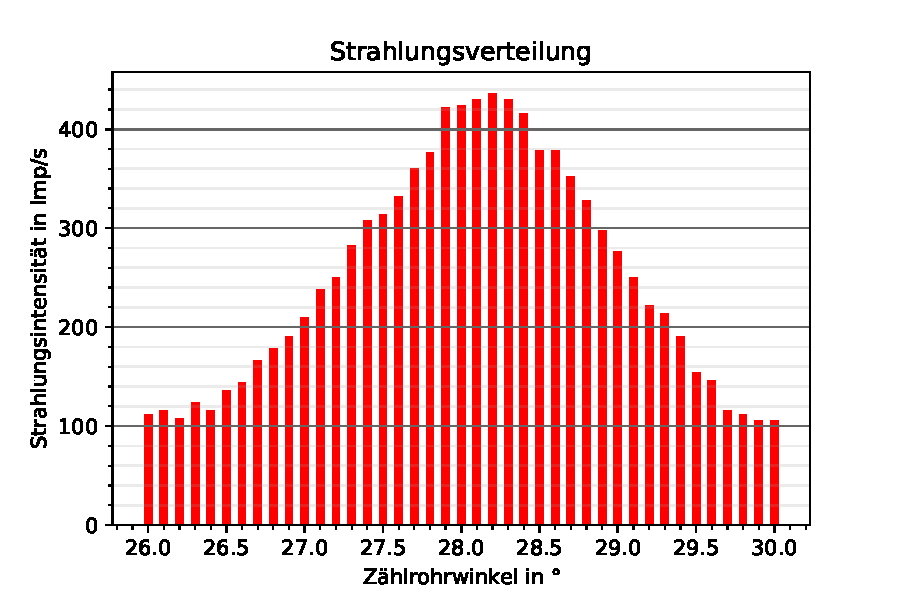
\includegraphics{Braggwinkel.pdf}
    \caption{Strahlungsintensitäten nach Winkel}
    \label{fig:Braggwinkel}
  \end{figure}
  Das gemessene Maximum liegt bei 28,2°.

\subsection{Bestimmung der Full Width at Half Maximum}
Im Diagramm \autoref{fig:Emspektrum} sind die gemessenen Strahlungsintensitäten gegen die 
verschiedenen Wellenlängen aufgetragen worden, Im Diagramm \autoref{fig:EmspektrumII} gegen die Energien.
Die Punkte zeigen an welchen Stellen die verbundenen Messwerte genau liegen. Auf der ganz linken Seite sieht man Teile des Bremsberges, dessen 
maximale Energie bzw. minimale Wellenlänge kann hier nicht ersichtlich werden da im zugehörigen Winkelbereich nicht 
gemessen wurde. Darauf folgt die $K_\alpha-$ und dann ganz rechts die $K_\beta-$Linie, weleche jeweils als deutlicher
Peak erkennbar sind. In den Peaks sind bei der hälfte ihrer Höhe horizontale Linien eingezeichnet welche die halbe
Höhe der Peaks kennzeichnen. Die Peaks liegen an folgenden Stellen:
\begin{center}
  $K_\alpha -Peak: \lambda_\alpha=13,9086\si[]{nm},$  $E_{K\alpha}=8.914\si[]{KeV}$\\
  $K_\beta -Peak:  \lambda_\beta=15,4145\si[]{nm},$  $E_{K\beta}=8.043\si[]{KeV}$
\end{center} 
Die zugehörigen Halbwerte $K_{i,1/2}$ und Messpunkte $E_{i,j}$ $i\in\{\alpha,\beta\}$, $j\in\{+,-\}$ bei denen 
der Halbwert zum ersten mal überschritten bzw. wieder unterschritten wurde lauten:
\begin{center}
  $K_{\alpha,1/2}=799.5\si[]{Imp/s}$, $E_{\alpha,+}=8.9996\si[]{KeV}$, $E_{\alpha,-}=8.7484\si[]{KeV}$, $\Rightarrow$ $\Delta E_{FWHM\alpha}=0.2512\si[]{KeV}$\\
  $K_{\beta,1/2}=2525.0\si[]{Imp/s}$, $E_{\beta,+}=8.1118\si[]{KeV}$, $E_{\beta,-}=7.9102\si[]{KeV}$, $\Rightarrow$ $\Delta E_{FWHM\beta}=0.2015\si[]{KeV}$
\end{center}
Aus diesen Werten ergibt sich über $A=\frac{E_K}{\Delta E_{FWHM}}$ direkt das Auflösungsvermögen:
\begin{center}
  $A_\alpha=35.4835$\\
  $A_\beta=39.9101$
\end{center}


  \begin{figure}
    \centering
    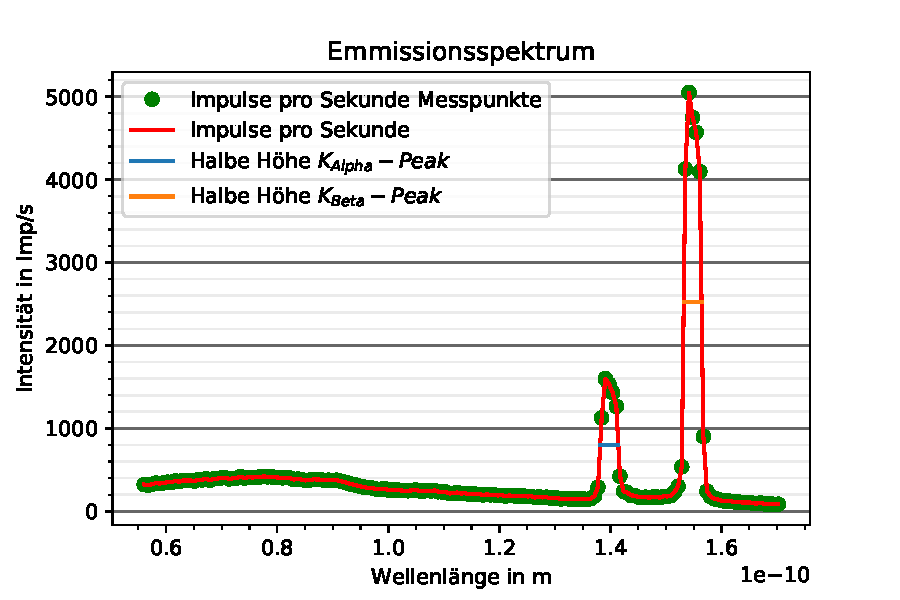
\includegraphics{Emmisionssprktrum.pdf}
    \caption{Intensitäten nach Wellenlänge}
    \label{fig:Emspektrum}
  \end{figure}

  \begin{figure}
    \centering
    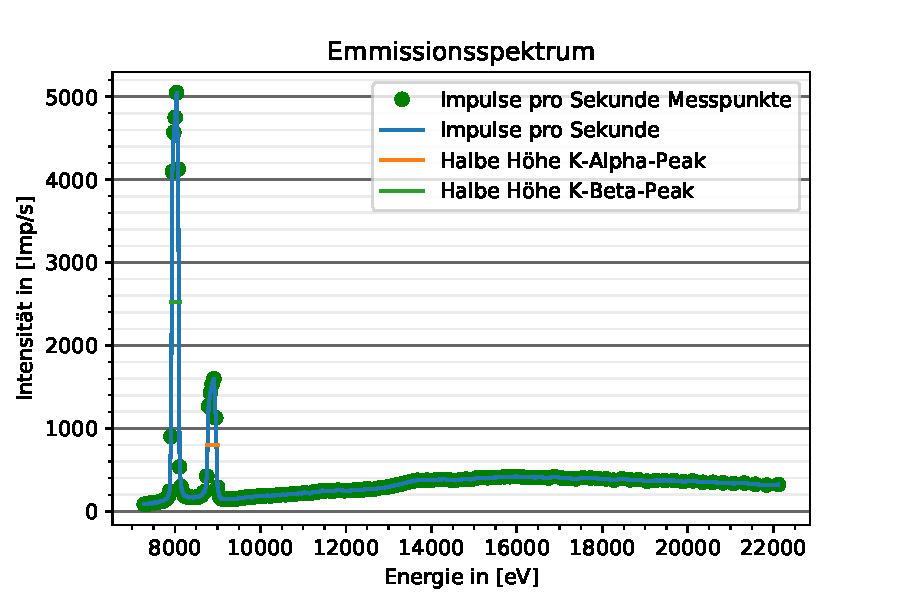
\includegraphics{EmmisionssprktrumII.pdf}
    \caption{Intensitäten nach Energie}
    \label{fig:EmspektrumII}
  \end{figure}

  \subsection{Bestimmung der Absorbtionskonstanten}
  Aus der NIST Datenbank wird die Abschirmkonstante $E_{K,abs}=  8.98796\si[]{KeV}$\\ übernommen. Durch sie kann
  über den Zusammenhang $\sigma=Z-\sqrt{\frac{E_{K,abs}}{R_\infty}}$, mit der Rydbergenergie $R_\infty=0.0136\si[]{KeV}$
  und der Ordnungszahl von Kupfer $Z=29$ sofort die Absorbtionskonstante $\sigma_1$ berechnet werden:
  \begin{center}
    $\Rightarrow \sigma_1=3.2924$
  \end{center}
  Nun lassen sich auch sofort mit $n=1$, $m=2$, $l=3$ die Abschirmkonstanten $\sigma_2$ und $\sigma_3$ bestimmen:
  \begin{center}
    $\sigma_2=z-(z-\sigma_1)m\sqrt{\frac{R_\infty +nE_{K,\alpha}}{nR_\infty}}$=11.0843\\
    $\sigma_2=z-(z-\sigma_1)l\sqrt{\frac{R_\infty +nE_{K,\alpha}}{nR_\infty}}$=2.1265\\
  \end{center}
  \subsection{Analyse der Absorberspektren}
  Als nächstes wurden die Absorberspektren verschiedener Elemente bestimmt. Dazu wurde aus dem Winkel $\Theta$ der Mitte der K-Kante mithilfe der Bragg-Bedingung die 
  zugehörige Energie $E_K$ und daraus die Absorbtionskonstante $\sigma_K$ berechnet. In den nachfolgenden Grafiken 
  \autoref{fig:EmspektrumIII},
  \autoref{fig:EmspektrumIV},
  \autoref{fig:EmspektrumV},
  \autoref{fig:EmspektrumVI},
  \autoref{fig:EmspektrumVII},
  \autoref{fig:EmspektrumVIII},
  sind die jeweiligen Maximal- und Minimalwerte $I_{max}$ und $I_{min}$
  aus welchen über die Beziehung $I_K=I_{min}+\frac{I_{max}-I_{min}}{2}$ die Mitte der K-Kante berechnet wurde. Anschließend wurde eine Gerade durch beide Punkte gelegt und anhand ihrer
  der Winkel $\Theta$ berechnet.
  \begin{table}
    \centering
    \label{tab:magnetfeld}
    \caption{Daten der Absorber}
    \sisetup{table-format=1.2}
    \begin{tabular}{S[table-format=3.2] S S S S S [table-format=3.2]}
      \toprule
      {Absorber} & {Ordnungszahl}&  {$\Theta$[°]} & {$E_K$[KeV]}& {$\sigma_K$[]}\\
      \midrule
      Brom      & 35  & 14.25 & 12.50 & 4.833\\
      Zirkonium & 40  & 10.75 & 16.50 & 5.659\\
      Zink      & 30  & 19.35 & 9.29  & 4.071\\
      Strontium & 38  & 11.65 & 15.24 & 4.939\\
      Rubidium  & 37  & 12.25 & 14.51 & 4.724\\
      Gallium   & 31  & 18.75 & 9.58  & 4.698\\

      \bottomrule
    
    \end{tabular}
  \end{table}
  
  \begin{figure}
    \centering
    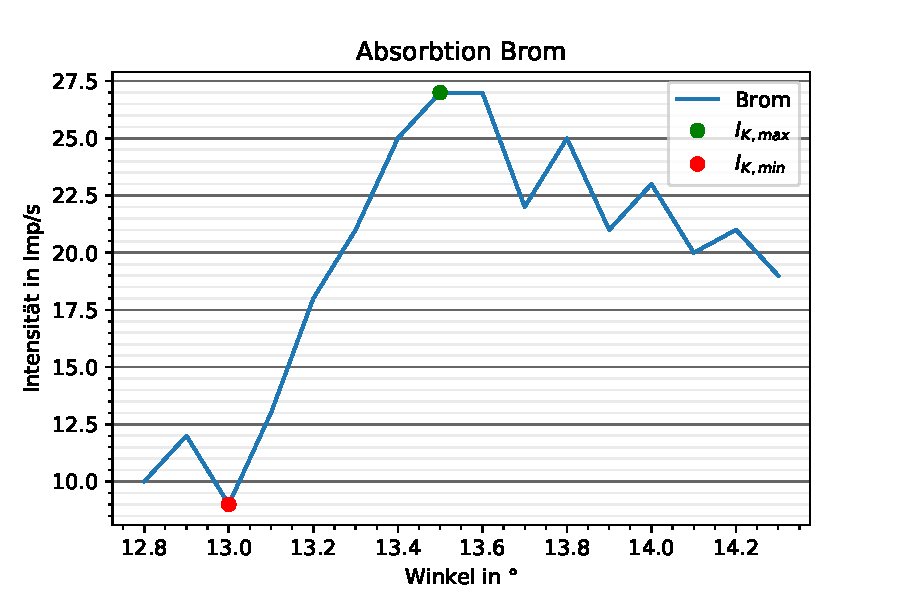
\includegraphics{AbsorbtionsspektrumBrom.pdf}
    \caption{Intensitäten nach Winkel eines Brom-Absorbers}
    \label{fig:EmspektrumIII}
  \end{figure}

  \begin{figure}
    \centering
    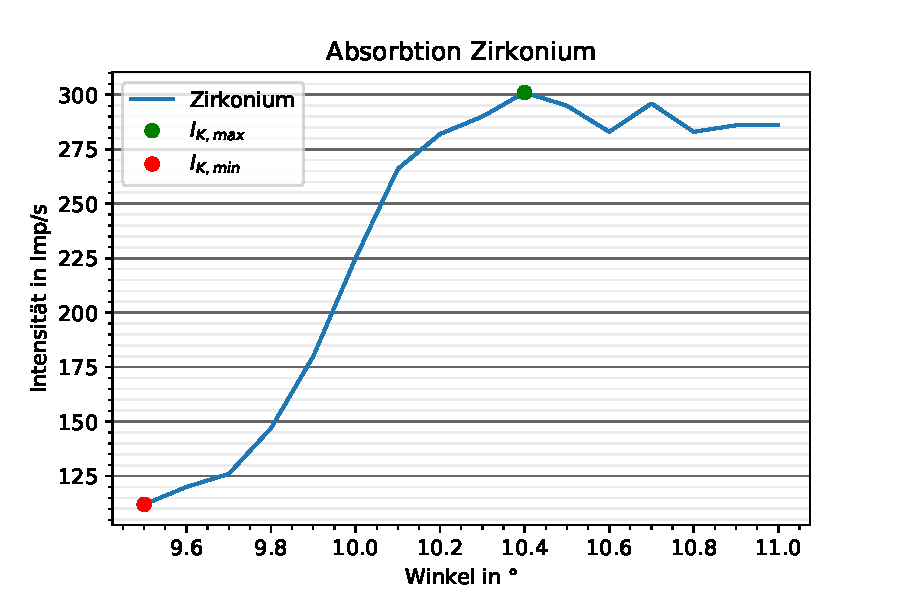
\includegraphics{AbsorbtionsspektrumZirkonium.pdf}
    \caption{Intensitäten nach Winkel eines Zirkonium-Absorbers}
    \label{fig:EmspektrumIV}
  \end{figure}

  \begin{figure}
    \centering
    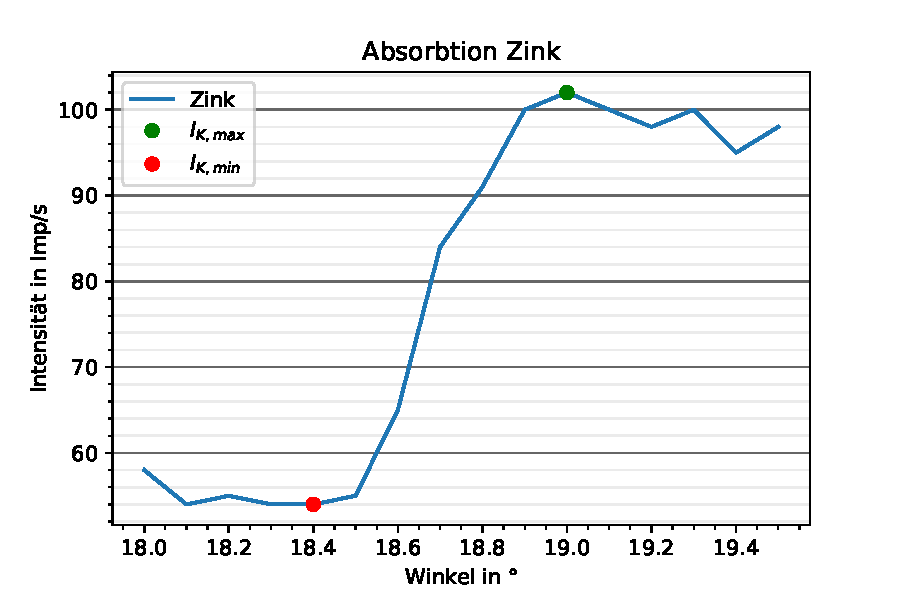
\includegraphics{AbsorbtionsspektrumZink.pdf}
    \caption{Intensitäten nach Winkel eines Zink-Absorbers}
    \label{fig:EmspektrumV}
  \end{figure}

  \begin{figure}
    \centering
    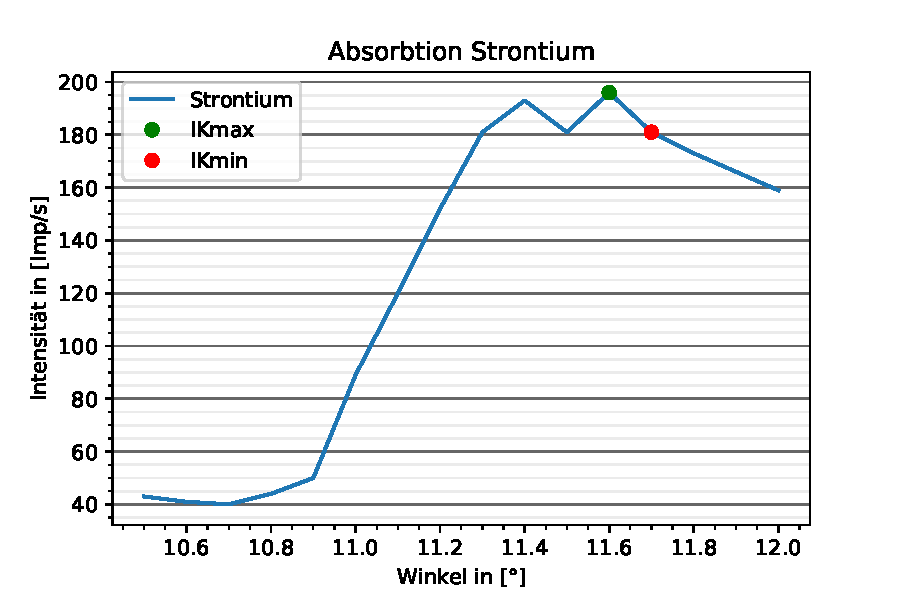
\includegraphics{AbsorbtionsspektrumStrontium.pdf}
    \caption{Intensitäten nach Winkel eines Strontium-Absorbers}
    \label{fig:EmspektrumVI}
  \end{figure}

  \begin{figure}
    \centering
    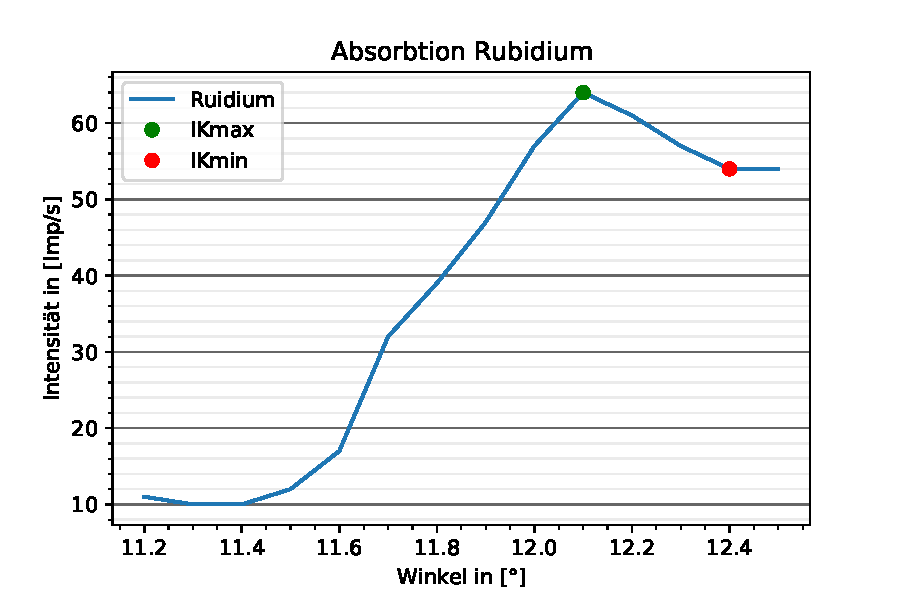
\includegraphics{AbsorbtionsspektrumRubidium.pdf}
    \caption{Intensitäten nach Winkel eines Rubidium-Absorbers}
    \label{fig:EmspektrumVII}
  \end{figure}

  \begin{figure}
    \centering
    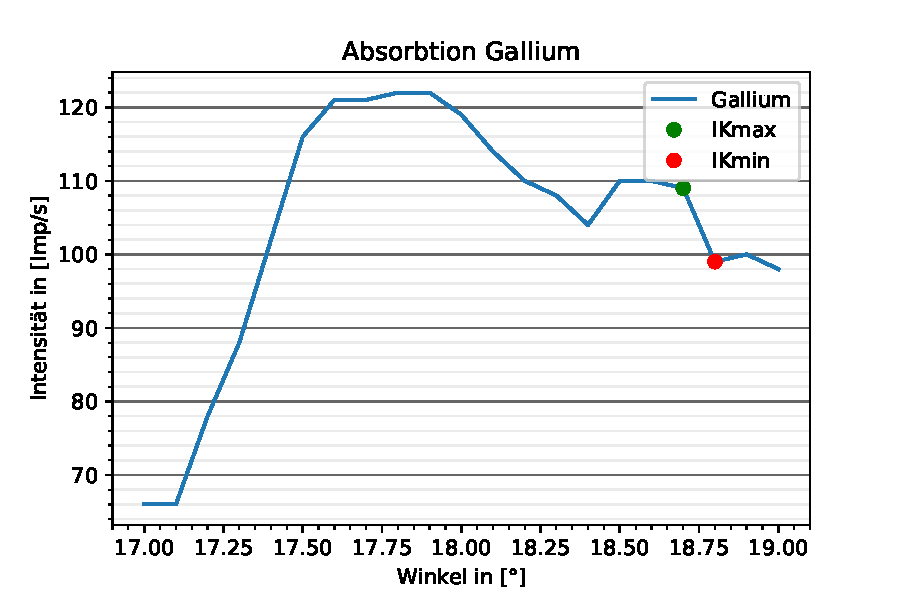
\includegraphics{AbsorbtionsspektrumGallium.pdf}
    \caption{Intensitäten nach Winkel eines Gallium-Absorbers}
    \label{fig:EmspektrumVIII}
  \end{figure}
